\documentclass[letterpaper, 8pt]{extarticle}
\usepackage{amssymb,amsmath,amsthm,amsfonts}
\usepackage{multicol,multirow}
\usepackage{calc}
\usepackage{ifthen}
\usepackage[landscape]{geometry}
\usepackage[colorlinks=true,citecolor=blue,linkcolor=blue]{hyperref}
\usepackage{booktabs}
\usepackage{ulem}
\usepackage{enumitem}
\usepackage{tabulary}
\usepackage{graphicx}
\usepackage{siunitx}
\usepackage{tikz}
\usepackage{derivative}
\usepackage{svg}
\usepackage{listings}
\usepackage{color}
\usepackage{soul}
\usepackage{clrscode3e}
\usepackage{setspace}
\usepackage{tikz}

\setstretch{0.5}
\setlength{\tabcolsep}{2.0pt}

\ifthenelse{\lengthtest { \paperwidth = 11in}}
    { \geometry{top=.25in,left=.25in,right=.25in,bottom=.35in} }
	{\ifthenelse{ \lengthtest{ \paperwidth = 297mm}}
		{\geometry{top=1cm,left=1cm,right=1cm,bottom=1cm} }
		{\geometry{top=1cm,left=1cm,right=1cm,bottom=1cm} }
	}

\newenvironment{Figure}
  {\par\medskip\noindent\minipage}
  {\endminipage\par\medskip}

\pagestyle{empty}
\makeatletter
\renewcommand{\section}{\@startsection{section}{1}{0mm}%
                                {-1ex plus -.5ex minus -.2ex}%
                                {0.5ex plus .2ex}%x
                                {\normalfont\normalsize\bfseries}}
\renewcommand{\subsection}{\@startsection{subsection}{2}{0mm}%
                                {-1explus -.5ex minus -.2ex}%
                                {0.5ex plus .2ex}%
                                {\normalfont\small\bfseries}}
\renewcommand{\subsubsection}{\@startsection{subsubsection}{3}{0mm}%
                                {-1ex plus -.5ex minus -.2ex}%
                                {1ex plus .2ex}%
                                {\normalfont\tiny\bfseries}}
\makeatother
\setcounter{secnumdepth}{0}
\setlength{\parindent}{0pt}
\setlength{\parskip}{0pt plus 0.5ex}
% -----------------------------------------------------------------------
% \tymin=37pt
% \tymax=\maxdimen

% Custom siunitx defs
\DeclareSIUnit\noop{\relax}
\setlist[itemize]{noitemsep, leftmargin=*}
\setlist[enumerate]{noitemsep, leftmargin=*}

\NewDocumentCommand\prefixvalue{m}{%
\qty[prefix-mode=extract-exponent,print-unity-mantissa=false]{1}{#1\noop}
}

% Shorthand definitions
% \newcommand{\To}{\Rightarrow}
\DeclareMathOperator{\divv}{div}

% condense itemize & enumerate
\let\olditemize=\itemize \let\endolditemize=\enditemize \renewenvironment{itemize}{\olditemize \itemsep0em}{\endolditemize}
\let\oldenumerate=\enumerate \let\endoldenumerate=\endenumerate \renewenvironment{enumerate}{\oldenumerate \itemsep0em}{\endoldenumerate}
\setlist[itemize]{noitemsep, topsep=0pt, leftmargin=*}
\setlist[enumerate]{noitemsep, topsep=0pt, leftmargin=*}

\title{2GA3}

\begin{document}

\raggedright
\tiny

% \begin{center}
% 	{\textbf{COMPSCI 2GA3 Cheatsheet v1.0.0 (OSCS Edition)}} \\
% \end{center}
\setlength{\premulticols}{1pt}
\setlength{\postmulticols}{1pt}
\setlength{\multicolsep}{1pt}
\setlength{\columnsep}{2pt}
\begin{multicols*}{6}
   

	\section{Logic Basics}
	% \subsection{Physics}
	% \textbf{Ohm's Law:} $R = \frac{U}{T}$\\
	% \textbf{Series:} \\
	% $R_T = \sum_{i=1}^N R_i$ \\
	% $V_T = \sum_{i=1}^N V_i$ \\
	% $I_T = I_1 = I_2 = \dots = I_N$\\
	% \textbf{Parallel:} \\
	% $1/R = \sum_{i=1}^N (1/R_i)$\\
	% $V_T = V_1 = V_2 = \dots = V_N$\\
	% $I_T = \sum_{i=1}^N I_i$ \\

	\subsection{Transistors}
	MOSFETs have 4 components: Source, Gate, Drain, and Base

	\textbf{PNP/NMOS:} Is on when gate is positive. No circle. \\
	\textbf{NPN/PMOS:} Is on when gate is negative. Has circle.

	Generally, transistors are used to pull the output to either
	a positive voltage, or a zero voltage (1 or 0, on or off).
	If output is not pulled to one of these,
	the output is floating and is indeterminate in voltage.

	\includegraphics[width=\linewidth]{transistor-types.png}

	\subsection{Logic Circuits}
	\subsubsection{Symbols (bottom have 2 inputs)}

	% \begin{center}
	% 	\begin{tabulary}{\linewidth}{@{}LL|LLLLLL@{}}
	% 		\toprule
	% 		p & q & and & nand & or & nor & xor & inv p \\
	% 		\midrule
	% 		1 & 1 & 1   & 0    & 1  & 0   & 0   & 0        \\
	% 		1 & 0 & 0   & 1    & 1  & 0   & 1   & 0        \\
	% 		0 & 1 & 0   & 1    & 1  & 0   & 1   & 1        \\
	% 		0 & 0 & 0   & 1    & 0  & 1   & 0   & 1        \\
	% 		\bottomrule
	% 	\end{tabulary}
	% \end{center}

	\begin{center}
		\includegraphics[width=.8\linewidth]{logic-gates.png}
	\end{center}
	\subsubsection{Adders}
	Left: Half-adder. Right: Full-adder.
	\begin{center}
		\includegraphics[width=.5\linewidth]{half-adder.png} \\
		\includegraphics[width=.9\linewidth]{full-adder.png} \\
		% \includegraphics[width=0.8\linewidth]{n-adder.png}
	\end{center}
	% REVIEW: Is there anything else that needs to be added here?
	Unlike half-adders, full-adders can receive carry-in bits.
	To add more bits, chain multiple full-adders together.
	If final carry at end is 1, there's an overflow error.

	\subsubsection{Latches \& Flip-flops}
	\textbf{Flip-flop}
	Every time the input switches from 0 to 1, the output switches to
	the opposite.
	% TODO: Add more detail about flip-flops

	% \includegraphics*[width=\linewidth]{flipflop.png}

	\textbf{Gated D-latch} \\
	\begin{center}
		\includegraphics[width=.6\linewidth]{gated-d-latch.png}
		\begin{tabulary}{\linewidth}{@{}CC|CCL@{}}
			\toprule
			$E/C$ & $D$ & $Q$               & $\overline{Q}$               &   \\
			\midrule
			0     & X   & $Q_\textit{prev}$ & $\overline{Q}_\textit{prev}$ & No change \\
			1     & 0   & 0                 & 1                            & Reset     \\
			1     & 1   & 1                 & 0                            & Set       \\
			\bottomrule
		\end{tabulary}
	\end{center}
	\begin{itemize}
		\item Q - The stored bit
		\item D - Data/bit to write to Q
		\item E - The enabler (Must be 1 to enable writing, otherwise nothing changes)
		\item Operate on the principle of propagation delay.
		\item Stacking many of them can be used to create a register:
	\end{itemize}

	% REVIEW: Do we need this?
	% seems like a lot of space dedicated to something that's trivial to derive
	% from scratch
	\includegraphics[width=\linewidth]{register.png}

	\subsection{Counters}
	For each transition from \textbf{low to high}, the counter increments
	the binary output by 1. (Counting the transition from high to low does
	the same thing, but the lecture used rising-edge counters).

	\subsection{Propagation Delay}
	The rate at which a transistor switches. Typical 100 ps (picoseconds)
	\subsection{Decoders}
	Take in an $n$-bit number, and turn on one of $2^n$ outputs.

	\subsection{Feedback Loops}
	\includegraphics[width=\linewidth]{Feedback_loop.png}
	\begin{itemize}
		\item Counter increments each time the clock changes from 0 to 1
		\item Decoder moves to the next instruction each time
		\item Stop sends a signal back to the and gate which stops counter
	\end{itemize}

	\subsection{Multiplexer / Demultiplexer}
	\textbf{Multiplexer} turns $n$ signals into a single signal. Chooses
	which signal to let through. \textbf{Demultiplexer} turns a single signal
	into $n$ signals. The single signal chooses which signal to output.

	\subsection{Software vs Hardware Design}
	Unlike software, which uses iteration, hardware uses replication. The advantages of replication are increased elegance, higher speed, and increased reliability.
	Hardware also uses gate minimization, abstraction and power optimization.

	\subsection{Fixed \& Programmable Logic}
	\textbf{Fixed logic circuits:} Pre-determined function.
	\textbf{Programmable logic:} FPGAs (reprogrammable, but still a significant cost to switching functions).
	\textbf{Stored program and re-programmable circuits:} Your computer right now.
	\section{Data Encoding}
	1 Byte = 8 bits.
	1 \textbf{Byte} encodes a character, integer, or pointer.
	1 \textbf{Word} is $n$ bytes, determined by the architecture.

	\subsection{Converting between bases}
	\textbf{Base 10 to Base N}
	Divide decimal \# by \# of new base.
	Take remainder as rightmost digit.
	Divide quotient of previous divide by new base.
	Repeat until quotient is zero.
	\textbf{Base N to Base 10}
	Take each column position of each digit, zero indexed, as $n$.
	For each column, do $c \cdot b^n$, where $c$ is the value of the column,
	and $b$ is the base value in base 10.

	\textbf{Important bases table}
	\begin{center}
		\begin{tabular}[!ht]{@{}lll@{}}
			\toprule
			Hex & Bin  & Dec \\
			\midrule
			0   & 0000 & 0   \\
			1   & 0001 & 1   \\
			2   & 0010 & 2   \\
			3   & 0011 & 3   \\
			4   & 0100 & 4   \\
			5   & 0101 & 5   \\
			6   & 0110 & 6   \\
			7   & 0111 & 7   \\
			\bottomrule
		\end{tabular}
		\begin{tabular}[!ht]{@{}lll@{}}
			\toprule
			Hex & Bin  & Dec \\
			\midrule
			8   & 1000 & 8   \\
			9   & 1001 & 9   \\
			A   & 1010 & 10  \\
			B   & 1011 & 11  \\
			C   & 1100 & 12  \\
			D   & 1101 & 13  \\
			E   & 1110 & 14  \\
			F   & 1111 & 15  \\
			\bottomrule
		\end{tabular}
	\end{center}

        \textbf{Important Bytes Table}
        \begin{center}
            \begin{tabulary}{\linewidth}{@{}LLL@{}} \toprule
                1 Byte              &          & 8 Bits \\
                1024 Bytes          & $2^{10}$ & 1 Kilobyte (KB) \\
                1024 Kilobytes (KB) & $2^{20}$ & 1 Megabyte (MB) \\
                1024 Megabytes (MB) & $2^{30}$ & 1 Gigabyte (GB) \\
                \bottomrule
            \end{tabulary}
        \end{center}

	\subsection{Fraction to Binary}
	\begin{enumerate}
		\item Let $x$ be the decimal part of our fraction.
		\item Let $b$ be our binary output.
		\item Multiply $x$ by 2.
		\item If $x \ge 1$, subtract 1 from $x$ and append 1 to $b$.
		\item If $x < 1$, append 0 to $b$.
		\item Goto step 3 until $x != 0$.
	\end{enumerate}

	\subsection{Signed Integers}
	\begin{itemize}
		\item \textbf{Two's complement:} Flip all bits, add 1.
		      Range is $-(2^{n-1}), +(2^{n-1} - 1)$
		\item \textbf{Sign-magnitude:} First bit is sign, rest is magnitude.
		      Range is $-(2^{n-1} - 1), +(2^{n-1} - 1)$.
		\item \textbf{One's complement:} Flip all bits.
		      Eg, +6 is $0110$, so to get -6 go from $0110 \to 1001 \to 1010$.
		      This has 2 zero, positive and negative zero.
		      Range is $-(2^{n-1} - 1), +(2^{n-1} - 1)$.
	\end{itemize}

	\subsection{Cast from Ints}
        \textbf{from smaller into to bigger ints} \\
	\textbf{sign-magnitude}: Copy the MSB to the bigger ints MSB. Then take the remaining bits and fill them from the right to left. \\
	\textbf{one's complement and two's complement}:
	Copy the Lowest order bits (the bits except the sign defining bit) and copy them to the other ints lowest order bits. \\
	Take the MSB and make all the remaining bits in the new int the MSB.
	\subsection{IEEE-754 Floats}
	Can represent values from $2^{-126}$ to $2^{127}$ which is $10^{-38}$ to $10^{38}$ in decimal.
	If double precision is used then the range is $2^{-1022}$ to $2^{1023}$ which is $10^{-308}$ to $10^{308}$ in decimal.
	Separated into \textbf{sign, exponent, and mantissa}.
	Entire float is represented in binary, and the exponent is biased by $2^{b-1} - 1$,
	where $b$ is the number of exponent bits.
	Leading 1 is dropped from mantissa.
	To calculate from IEEE, do $1.(m_2) \times 2^{(e_2)}$.
	(Convert out of base 2 first).
	Range is approximately $2^{(-2^b)+2}, 2^{2^b-1}$,
	where $b$ is the bits dedicated to the exponent, \textbf{minus 1}.
	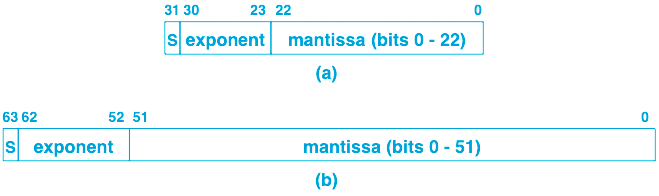
\includegraphics[width=\linewidth]{ieee-754.png}

	\subsubsection{Special Values}
	\begin{center}
		\begin{tabular}[!ht]{@{}cc|c@{}}
			\toprule
			Exponent & Mantissa   & Value        \\
			\midrule
			all 1s   & all 0s     & $\pm \infty$ \\
			all 1s   & not all 0s & NaN          \\
			all 0s   & not all 0s & denormalized \\
			all 0s   & all 0s     & $\pm 0$      \\
			\bottomrule
		\end{tabular}
	\end{center}

	\subsection{Binary-coded decimals}
	Instead of representing decimals using a float,
	use an arbitrarily long string of bytes, usually as binary ints.
	Efficiency can be improved using packed BCDs, by putting 2 ints in one byte
	(each digit occupying a nibble).
	\verb|0x2D| is used by the textbook to represent a negative, placed at the end of the BCD.
	For a packed BCD, drop the 2.

	\subsection{Endianess}
	\textbf{Endian:} The way in which words(group of bytes) are stored in memory.
	\textbf{Big Endian:} Most significant byte first.
	\textbf{Little Endian:} Least significant byte first.
	Little endian is the most common method of storing data in memory.
	\includegraphics[width=\linewidth]{endianness.png}
	% \subsection{ASCII and Unicode}
	% \textbf{ASCII:} 128 characters, 7 bits.
	% \textbf{Unicode:} 1,114,112 characters, 21 bits. Has variable length encoding for optimization i.e has as many bytes as needed.
	% \subsection{Unicode Encoding}
	% \includegraphics*[width=\linewidth]{unicode.png}



	\subsection{Types of architecture}
	\textbf{Von Neumann architecture (left):}
	\begin{itemize}
		\item Single memory block which contains both instructions and data.
		\item Offers complete flexibility: at any time, owner can change how much of the memory is devoted to programs and how much to data.
		\item More popular.
	\end{itemize}
	\textbf{Harvard architecture (right):}
	\begin{itemize}
		\item 2 separate memory. One is used for instruction, one is used for data.
		\item Inflexible, as you cannot use part of the instructional memory to store data and vise versa.
		\item Less popular. Sometimes used in small embedded systems.
	\end{itemize}
	\includegraphics[width=0.49\linewidth]{vn-arch.png}
	\includegraphics[width=0.49\linewidth]{harvard-arch.png}
	\subsubsection{Von Neumann Bottleneck}
	On computers running Von Neumann Architecture, time spent accessing memory can limit performance.
	To avoid the bottleneck, designs are chosen where operands are moved to registers instead of system memory.

	\subsection{Types of processors}
	A processor is a digital device that can perform a computation involving multiple steps. \\
	\textbf{Categories based on logic:} \\
	\begin{itemize}
		\item \textbf{Fixed logic}: Function fixed in hardware, performs a single task
		\item \textbf{Selectable logic}: Choose one of several fixed functions.
		\item \textbf{Parametrizable logic}: Accepts a set of parameters that control the computation of fixed functions.
		\item \textbf{Programmable logic}: list of instructions provided at runtime (you can code them)
	\end{itemize}

	\textbf{Categories based on Complexity:} \\
	\begin{itemize}
		\item \textbf{Co-processors}: Dedicated function. Usually performs a single task at high speed. Used in -> Floating point accelerator. Fixed/Selectable logic.
		\item \textbf{Microcontrollers}: Direct hardware control. Used in -> Elevator doors. Programmable logic.
		\item \textbf{Embedded System Processors}: real-time OS, dedicated hardware. usually more powerful than microcontrollers. Used in -> smart phone Programmable logic.
		\item \textbf{General-purpose Processors}: compatible for multiple systems. Used in -> CPU in a PC. Programmable logic.
	\end{itemize}

	\subsection{Parts of a processor}
	\begin{itemize}
		\item \textbf{Controller}: Responsible for program execution. Steps through the program and coordinates the actions of all other units.
		\item \textbf{Arithmetic logic unit}: Performs all computational tasks. Performs one operation at a time according to controller.
		\item \textbf{Local storage (registers)}: Hold data values such as operands for arithmetic operations and the result.
		\item \textbf{Internal connections}: Transfers data values between units, like from local storage to the ALU. AKA data paths/Bus/Control lines
		\item \textbf{External interface}: Handles all communication between the processor and the rest of the computer system.
	\end{itemize}

	\subsection{Fetch execute cycle}
	There is a \textbf{instruction pointer} which moves through the program performing every step. The cycle never ends while the system is running.
	\begin{enumerate}
		\item Fetch the next instruction
		\item Decode the instruction and fetch operands from registers
		\item Perform the arithmetic operation specified by the \textbf{opcode}
		\item Perform memory read or write, if needed
		\item Store the result back to the registers
		\item go to next instruction, Repeat forever.
	\end{enumerate}

	\subsection{Program Translation}
	\includegraphics[width=\linewidth]{program-translation.png}
	\begin{itemize}
		\item \textbf{Preprocessor:} Expands macros, producing modified source program.
		\item \textbf{Compiler:} Translates it to assembly.
		\item \textbf{Assembler:} Translates it to relocatable object code which contains references to external library functions.
		\item \textbf{Linker:} Replaces external function references with its code.
	\end{itemize}

	% Needs review and addition of more details maybe
	% \subsection{Fetch execute cycle notes}
	% \begin{itemize}
	% 	\item Instructions are stored as binary data defined in a instruction set.
	% 	\item The program starts at a constant point in memory which could be 0 or any other point, that part of memory should always have the necessary instructions to boot the system.
	% 	\item Fetch execute cycle runs indefinitely, that's why in general purpose computers an OS is running at all times that manages the execution of programs.
	% \end{itemize}


	\subsection{CISC vs RISC}
	\textbf{CISC}
	\begin{itemize}
		\item Each instruction performs a complex operation
		\item Instructions may take multiple clock cycles
		\item Fewer instruction calls
	\end{itemize}
	\textbf{RISC}
	\begin{itemize}
		\item Each instruction performs a simple operation
		\item Instructions all take the same number of clock cycles
		\item Many instruction calls needed
		\item Allows for pipelining, as each part of the instruction takes the same amount of time
	\end{itemize}

	\subsection{Pipelines}
	Allow for more than one instruction to be ``processed'' at the same time.
	Generally 5 stages:
	\begin{enumerate}
		\item Fetch next instruction
		\item decode \& fetch operands
		\item perform arithmetic operation
		\item read or write memory
		\item store result
	\end{enumerate}

	\subsubsection{Pipeline Stalls}
	Also known as hazards. 3 main types:
	\begin{itemize}
		\item
		      \textbf{Data Hazards:} Waiting for data from an earlier instruction.
		      Can be dealt with using data forwarding (allowing data to be used
		      before it exits the pipeline), re-arranging instruction order.
		\item
		      \textbf{Control Hazards:} Incorrect instruction is in the pipeline.
		      Occurs during jump instructions/branching. Jumps are not executed
		      until the fifth stage, so instructions directly after are fetched
		      inside the pipeline.  Can be dealt with using conditional branch
		      prediction, flushing pipeline if prediction is wrong.
		\item
		      \textbf{Structural Hazards:} Resource conflict (usually from external
		      source) (eg somebody else is accessing the same register bank). Can
		      be dealt with by loading data in parallel, eg using multiple banks.
	\end{itemize}
	\includegraphics[width=\linewidth]{stall-example.png}

	\subsection{Branching}
	Moving the instruction pointer to a different location in program.
	Can be either absolute branch, or relative branch.
	Branch prediction can be used to try to run code from a branch before
	the processor has the data needed to evaluate it, speeding up runtime.
	% REVIEW: idk what else needs to be added here,
	% this seems pretty trivial

	\section{Instruction Sets}
	Generally has the following parts:
	Operation number, registers, offset.
	\begin{itemize}
		\item \textbf{Opcode (operation code)}:
		      Specifies the operation to be performed.
		\item \textbf{Registers}:
		      Specifies the operands and the destination.
		\item \textbf{Offset}:
		      Think of it like array indexes. Can be a signed integer to
		      move backwords.
	\end{itemize}
	\includegraphics[width=\linewidth]{isa-example.png}

	\subsection{Design choices}
	\subsubsection{Encoding length}
	\textbf{Variable-length} encoding can improve instruction density,
	but \textbf{fixed-length} instructions are simpler to implement in hardware,
	and are thus more performant. Unused bits are ignored by the instruction.

	Offsets are used to encode immediate values (generally used for jumping).

	\subsubsection{Number of Operands}
        \begin{itemize}
    	\item \textbf{Zero operands:} Stack architecture, using push and pop. All operands are implicit.
    	\item \textbf{One operand:} Implicit destination (usually a special accumulator register)
    	\item \textbf{Two operands:} Specified destination, but uniary operations (eg \verb|add rA, rB #rA=rA+rB|)
    	\item \textbf{Three operands:} Specified destination, binary operations
        \end{itemize}
        TL;DR, more operands = more flexible instructions, but more space taken up by operands

	\subsubsection{Implicit vs Explicit Encoding}
        \begin{itemize}
    	\item \textbf{Implicit Encoding:} Operand types are always the same for a given opcode. Different opcodes are used for different types.
    	\item \textbf{Explicit Encoding:} Operand field specifies what type of operands are being provided.
        \end{itemize}

	\subsubsection{Operand Adressing Modes}
	\includegraphics[width=\linewidth]{operand-addressing-modes.png}

	% \subsubsection{Orthogonality}
	% Each instruction should perform a \textit{unique task},
	% without duplicating or overlapping the functionality of other instructions.
	% \textbf{Advantages}: Orthogonal instructions can be understood more easily,
	% and programmers don't need to pick between functions that perform the same task.

	% \subsection{Registers}
	% \begin{itemize}
	% 	\item
	% 	      \textbf{General Registers}:
	% 	      Fixed size (usually 32 or 64 bits), 2 basic ops, fetch and store.
	% 	      Numbered from 0 to $N-1$.
	% 	\item
	% 	      \textbf{Floating Point Registers}:
	% 	      Separate set of registers holding floats, but numbering overlaps.
	% 	      Floating point registers are automatically used if instruction requires FP.
	% 	\item
	% 	      \textbf{Special Registers}:
	% 	      \begin{itemize}
	% 		      \item
	% 		            \textbf{Program Counter (\textit{pc})} - Stores the address of the
	% 		            next instruction to fetch.
	% 		      \item
	% 		            \textbf{Comparer (\textit{cmp})} - Stores the result of the last
	% 		            comparison operation. (1 for true, 0 for false).
	% 		      \item
	% 		            \textbf{Accumulator (\textit{acc})} - For zero and one-operand
	% 		            architectures to store the result of the last command.
	% 	      \end{itemize}
	% \end{itemize}

	\subsubsection{Subroutines and Register Windows}
	When calling a subroutine, a window viewing the registers will shift between addresses,
	making some registers of them inaccessible, some new registers available,
	and keeping some between both calls.
	This allows for values to be passed to and from the subroutine,
	while keeping some values separated.
	\includegraphics[width=\linewidth]{register-windows.png}

	\subsubsection{Register Banks}
	\begin{itemize}
		\item Allows parallel access within same clock cycle $\to$ efficiency
		\item Some operations require operands from banks
		\item Register bank conflicts
	\end{itemize}

	\subsubsection{Register Conflicts}
	Accessing 2 registers from the same bank simultaneously causes a register conflict.
	Best case, it causes a stall in the pipeline. Worst case, it causes the system to crash. \\
	\subsubsection{Solution}
	\begin{itemize}
		\item reassign
		\item moving registers
		\item insert an instruction to copy values to the opposite register.
	\end{itemize}

	\section{Physical Implementation}
	\begin{center}
        \includegraphics[width=\linewidth]{data-paths.png}
	    \includegraphics[width=0.5\linewidth]{m1m2m3.png}
	\end{center}
	\begin{itemize}
		\item Core loop between M1, 32-bit pgm. ctr., 32-bit adder
		\item Instruction memory returns instruction at given address
		\item Instruction decoder takes instruction and decodes it into individual parts
		\item Register fields used to select registers used in instructions, register unit takes fields and returns contents
		\item M2 Multiplexer takes auxiliary adding functions (such as adding an offset) and passes it through ALU
		\item ALU performs operation. For addresses, it's passed directly to data memory to get data out,
		      for operations, data is passed to multiplexer to be stored into register for future use.
	\end{itemize}

    \section{Bit Representations}
    \includegraphics[width=\linewidth]{bitbit.png}

    \section{Microcode}
    Allows for simpler hardware design by offloading complexity to software.
    Macro instructions are made of microcode. 
    Have a different instruction set available internally.
    Microcontrollers(s) sprocess microcode to emulate macrocode.
    
    \subsection{Pros}
    Less prone to errors compared to hardware design.
    Easier to implement.
    Ease of extension and modification.
    Offers another level of abstraction.
    \subsection{Cons}
    More overhead than dedicated hardware design.
    Variable cost for macro instructions, depends on number of micro instructions in its implementation.
    Microcontroller needs to run very fast.

    \subsection{Vertical Microcode}
    Microcontroller is a centralized unit sequentially excuting code; controls a single functional unit at a time. It must be fast. Think of a macrocode instruction as a function composed of micro instructions run one at a time.

    \subsection{Horizontal Microcode}
    Control \textbf{multiple} functional units simultaneously.
    Each instruction executes several operations in parallel.
    
    \section{Memory \& Caching}
    Memory designed to be hierarchical, with data copied into faster access levels as needed (acting as caching layers): \\
    ALU $\to$ Registers $\to$ Memory $\to$ Storage.

    \subsection{RAM Types}
    \textbf{SRAM:} Similar to a latch, high power consumption, low latency, high access speed. \\
    \textbf{DRAM:} Similar to a capacitor, low power consumption, higher latency, slower access. As time passes the charge dissipates and becomes 0. Requires a refresh circuit.

    \subsection{Measure of Mem performance}
    \begin{itemize}
        \item \textbf{Density} number of memory cells per square area of silicon. Memory density tends to double approximately every eighteen months. (Moore’s Law)
        \item \textbf{Read} and \textbf{write} performance.
        \item \textbf{Latency} Time taken to do one operation. A memory system may need extra time between operations, latency alone is insufficient.
        \item The \textbf{read cycle} time and \textbf{write cycle} time are used as measures of memory system performance because they assess how quickly the memory system can handle a sequence of requests.
    \end{itemize}
    
    Memory bus: interface width / word size / number of lines
    
    \subsection{Memory Addressing}
    Memory is word addressable (r/w ops apply to words), but virtual addresses at processor level are byte addresses. \\
    Let $b$ be the byte-address, and $N$ be the number of bytes in a word. Then 
    \begin{itemize}
        \item $\textbf{word address } w = \lfloor \frac{b}{N} \rfloor$ \\
        \item $\textbf{offset} = b \mod N$ \\
    \end{itemize}
    We use $N$ as powers of 2, to make arithmetic easier (division by $2^x$ is the same as right shiting by $x$ bits, Modulo equivalent to truncation at $x$ digits).
    
    \subsection{Byte Alignment}
    If a piece of data is stored in \textbf{a single word}, then it is said to be byte aligned. Good for performance.

    \subsection{Memory Address Space}
    Address size is the same as word size. \textbf{address space} is the set of possible addresses (An n-bit addressable system will have $2^n$ different memory addresses). If we use byte addressing instead of word addressing, we have a factor of $N$ less memory ($N = $ size of a word).
    % 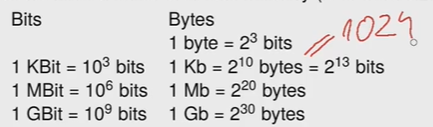
\includegraphics[width=0.9\linewidth]{bytes_bits.png}
    
    \subsection{Memory Management Unit}
    Interface that multiple memory chips can connect to, providing a common address space to processor.
    Implements virtual memory, caching.
    Combining address spaces generally done either sequentially or interleaved (generally \#2).
    Interleaving done by selecting the least significant bits, assuming $2^N$ different chips to distribute over.

    \subsection{Caching}
    The same data is frequently read / written to. It can also reduce the impact of the Von Neumann bottleneck.\
    L1 cache: associated with one particular core.
    L2 cache: on-chip cache that may be shared.
    L3 cache: on-chip cache that is shared by multiple cores.
    \textbf{Characteristics:}
    Small - size of cache $\ll$ size of data at producer.
    Active - contains algorithm that decides data to store and handles requests.
    Transparent - producer and consumer unaware of cache's existence.
    Automatic - self-contained.

    Hit ratio: $r = \frac{N_{\textit{hit}}}{N_{\textit{hit}} + N_{\textit{miss}}}$ \\
    Cache look up cost: $C_\textit{cache} = r C_h + (1 - r) C_m $

    Cache always improves performance when $C_m > C_h$ and $r > 0$.

    With two caches, $C_\textit{cache} = r_1 C_{h1} + r_2 C_{h2} + (1 - r_1 - r_2) C_m$

    \subsection{Replacement Policies}
    Least Recently Used, Least Frequently Used

    \subsection{Cache Maintenance Policies}
    \textbf{Write Through} - As soon as value is modified, update all caches.
    \textbf{Write Back} - Set a flag when modified (dirty bit), only write back when value in cache is evicted.

    \subsection{Cache Coherence Protocols}
    Multiple processors changing the same value means a cache coherence protocol is needed.
    All caches need to see write ops in same order, and need to be informed immediately when a value is changed. Some cases may lead to cache being flushed.
    Strategies: common directory, snooping % TODO: someone elaborate on these two types please

    \subsection{Direct Mapped Memory Cache}
    Several cache lines (blocks) containing words from memories.
    Broken up into Tags and Blocks (both in powers of 2). \\

    \begin{itemize}
        \item \textbf{Offset}: $o = a \mod W$, where $o$ is the offset, $a$ is the address, and $W$ is the number of words per line. (if $W = 2^x$ then $x$ lowest order bits in bin)
        \item \textbf{Block ID}: $b = (a \divv W) \mod B$, where $B$ is the number of blocks/lines in the cache.(if $B = 2^x$ then $x$ lowest order bits in bin excluding $o$)
        \item \textbf{Tag}: $t = (a \divv W) \divv B$ (everything else)
    \end{itemize}
    Total mem needed to implement cache (bytes) = no.of lines $\times$ no. of words per line $\times$ no.of bytes per word
    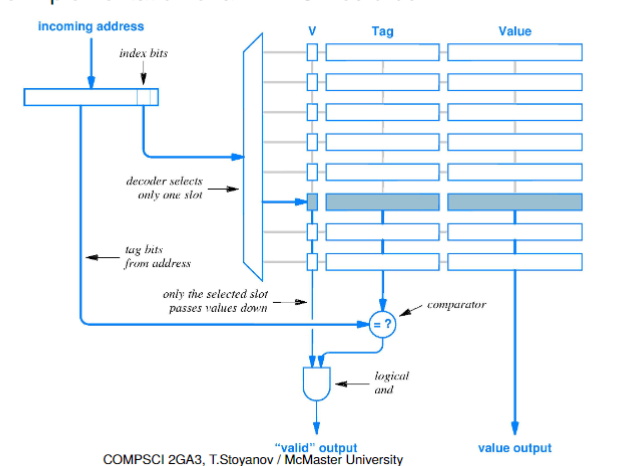
\includegraphics[width=\linewidth]{DMMC_hardware.png}

    \subsection{Set Associative Memory Cache}
    Maintains \textit{multiple} underlying caches, searches all of them simultaneously through parallelism.
    For a single DMMC, addresses which collide in a slot will lead to constant cache misses, but with set associative we can reduce the chance of this happening.
    Full parallelism = Content Addressable Memory (CAM).

    \subsubsection{Calculate bits for Tag ID}
    Assume a \textbf{16-bit architecture} where the cache can hold \textbf{8 blocks/lines} of memory, each which is \textbf{32 bytes long}. How many bits are needed to represent the tag id?
    \begin{itemize}
        \item 16-bit architecture - \textbf{2} bytes per word
        \item 8 blocks - $2^3$ blocks, so \textbf{3} bits for block id
        \item 32 bytes per block - $32 / 2 = 16 = 2^4$ words per block, so \textbf{4} bits for offset
        \item $16 - 3 - 4 = 9$ bits for the tag id.
    \end{itemize}
    
    \section{Virtual Memory}
    Addresses sent b/t CPU and MMU are in virtual address space, MMU talks to physical memory in physical address space.
    Keeps mapping between virtual space $i$ and a pair, \textit{(base, bound)}.
    \textit{base} points to mem address mapping to vaddress 0, \textbf{bound} can be scaled dynamically and points to end of memory space.
    We split memory space into variable sized chunks to allow us to "use" more memory than is available, as most memory is idle.
    
    \subsection{Demand Paging}
    Split program memory up into fixed size chunks called \textbf{pages}.
    Similar to segmentation, more straightforward to implement.
    Requires cooperation b/t software and hardware.
    \textbf{Software:} Configure hardware - monitor page use - move pages b/t memory and storage
    \textbf{Hardware:} Handle address mapping - record when a page is used - detect access attempt to a missing page

    \subsubsection{Process}
    1. MMU tries to load address $a$ on page $P$
    2. MMU checks page table $P_t[P]$. Check if \textit{presence bit} is set.
    2.5. If not, MMU raises page fault, OS handles fault and loads P from hard drive, if no space left OS swaps out page with \textit{use bit} of 0, if \textit{modified bit} is set, save page, otherise discard.
    3. If yes, MMU looks up address and updates \textit{use bit} and \textit{modified bit}.

    Page table holds pointers to frames, allocates all pages for program's memory space.
    Also maintains flags: presence bit (if page is resident), use bit (each time address is fetched, clear if page is unused for x cycles), modified bit (set if memory address in page has been written to)

    Accessing address $a$ with each page being $V$ bytes long:
    Page number is $N = a \divv V$. Frame address is $F = P_t[N]$. Offset: $O = a \mod V$. Physical address of $a$ is $F + O$.
    % insert image if we have space
    
    \subsection{Translation Lookaside Buffer}
    Type of cache, we keep a record of $F = P_t[N]$ so if we look it up again we can return the cached version.
    Parallel lookup through TLB and request to memory.
    Cache holds virtual addresses with process ID:
    [ID][Virtual Address] = [address used by cache]
    % TODO

    \section{IO Bus}
    A bus is a digital communication mechanism that allows two or more functional units to transfer control signals or data. Interconnects functional units (includes external devices). A bus standard must specify all the details needed to construct hardware. An access protocol must be defined to permit the sharing of a bus b/w parts. The access protocol specifies how an attached device can determine whether the bus is available or is in use, and how attached devices take turns using the bus.

    \subsection{Parallel vs Serial}
    \textbf{Parallel:} Multiple data lines, pretty straight forward, multiply lines and clockspeed to get throughput. Lower latency per word, can send in one go. Potentially higher throughput, but possible issues with interference.
    \textbf{Serial:} Single data line, clockspeed = throughput in bits. Higher latency (word sent sequentially), but possibly higher rate of data transfer.

    \subsection{Communication Directionality}
    Single direction: data can only flow in one direction, ever.
    Half duplex: one direction at a time.
    Full duplex: both directions at the same time.

    \subsection{Multiplexing}
    Take a bunch of bits to be transfered, resize them into chunks, pass them into mux hardware, demux at the other end and reassemble.
    % elaborate on this

    \subsection{Physical Implementation}
    Bus implemented from parallel wires along edge of board (eg PCIe).
    Different lines dedicated to different functions:
    \textbf{Control lines:} Take control of bus, request transfers, set signals and interrupts.
    \textbf{Address lines:} Transmit the address in a fetch/store operation.
    \textbf{Data lines:} Transmit data.

    Alternatively, multiplex using combined address and data lines together.
    All devices connected to bus see data, address, control bits sent, only device with matching address responds.
    Each device on bus has a unique address, with each address corresponding to particular device function.
    Each socket has a range pre-assigned.

    \subsection{Unified Address Space}
    IO devices are in same space as memory addresses. Fetch/store to device is same as fetch/store to memory. MMU manages address alloc and raises faults when accessing \textit{hole} in address space.

    \subsection{Bridging}
    Architecture has one primary bus and several aux busses.
    Bridges connect busses, provide address translation, relays data.
    Provides address translation in unified address space, addresses on main bus can be kept constant while being mapped differently on aux bus.
        
    \section{Interrupts}
    Two options for IO operations:
    \textbf{Option 1:}
    Each device exposed as an address.
    CPU performs fetch/store directly.
    Ops triggered and monitored by CPU.
    \textit{Programmed I/O}

    \textbf{Option 2:}
    Smart device carries out operations independently.
    Device must contain processor.
    CPU sets high-level goals, local processor performs the actual operations and monitors for results.
    \textit{Interrupt-driven I/O}

    \subsection{Programmed I/O}
    CPU takes control of all low-level operations on device.
    Device can be very simple, fixed logic circuits.
    Sync issues, as CPU runs at a high clock race but device operations are much slower. Result: CPU has to wait for device.
    Special registers on device used to exchange information: Control and Status Registers (CSRs).
    Control register corresponds to set of addresses that respond to a store operation.
    Status register corresponds to set of addresses that respond to fetch operation.
    Repeated polling is used to check for operation status.
    Inefficient, not commonly used today.
    
    \subsection{Interrupt-driven I/O}
    Requires special design for I/O device hardware (on-board processor and ability send interrupts), I/O bus architecture (interrupt signals), processor architecture (context switching), programming paradigm (OS supports interrupts).
    At boot time, fill IV table by device. IDs can either be by plug-in slot, or set by BIOS.
    Hotplug devices trigger interrupts, handler allocates device id and interrupt handler for new device.
    Handling usually done through device drivers.

    \subsubsection{Interrupt Vectors}
    Store a vector of interrupt response pointers in memory, so we know how to respond to each device's interrupt.
    % if we have space add an image of interrupt vectors

    \subsection{Device Drivers}
    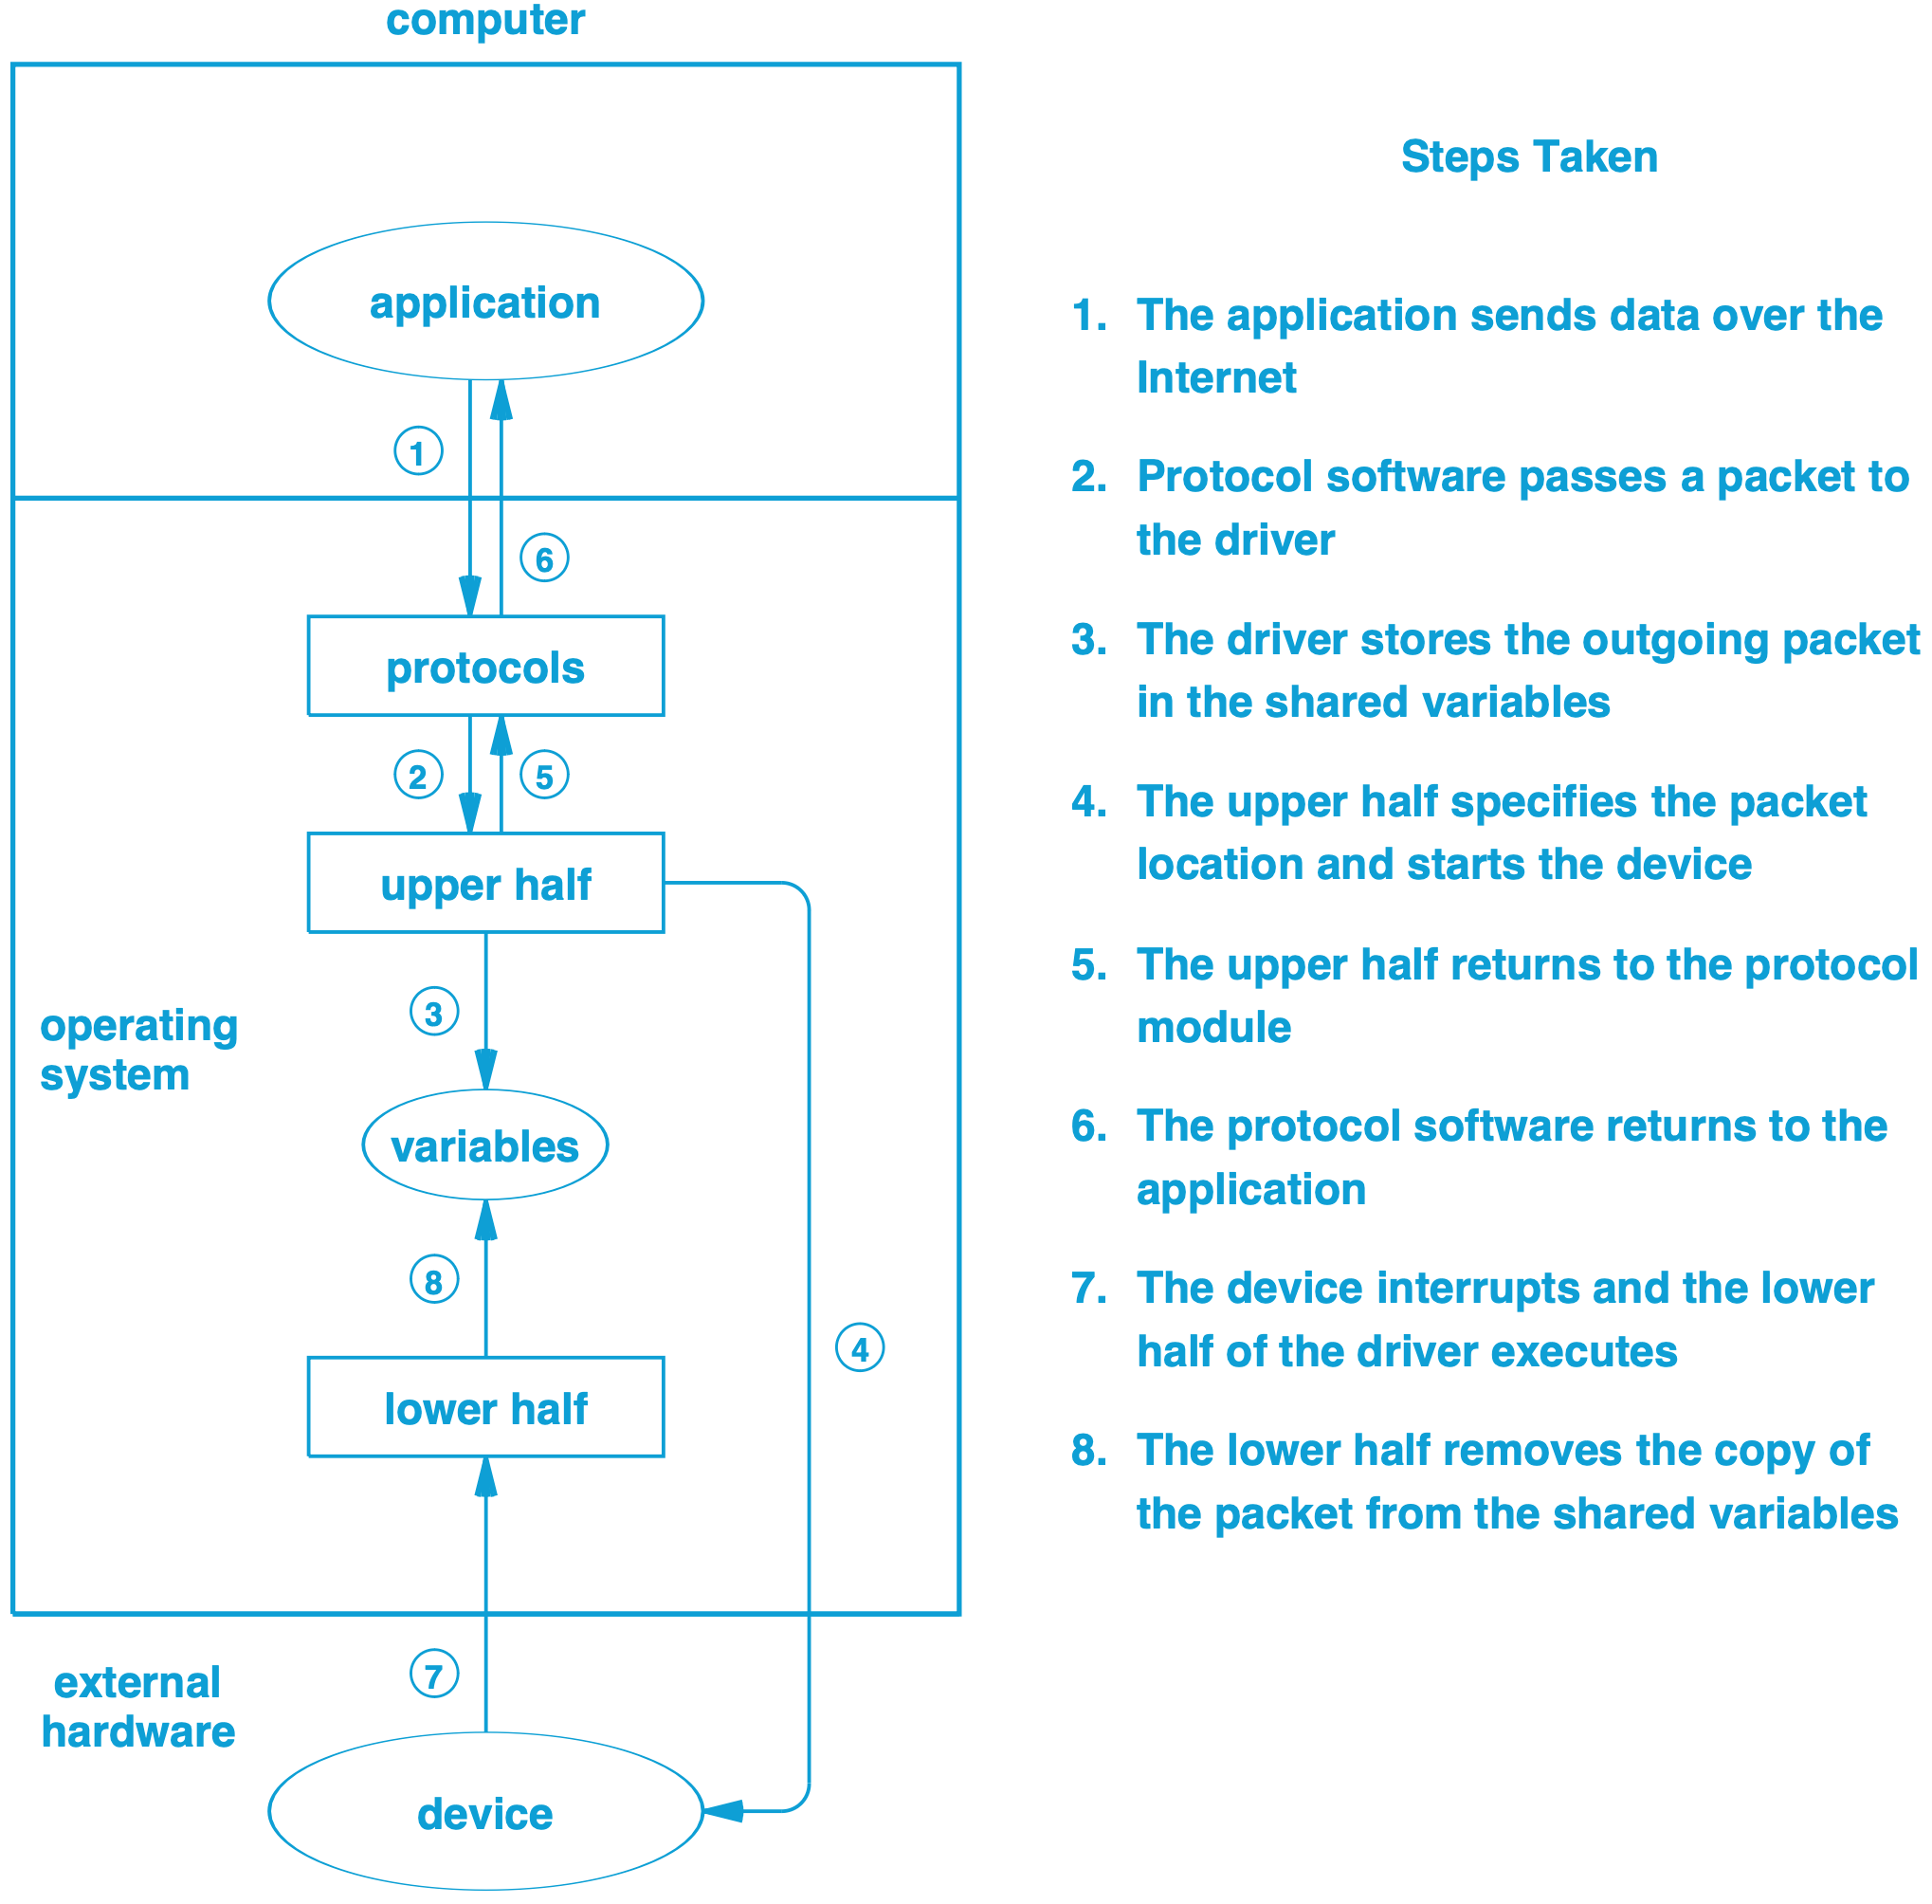
\includegraphics[width=\linewidth]{driver-halves.png}
    \textbf{Upper Half:} Provides OS interface to user-space programs (syscalls) \\
    \textbf{Lower Half:} Runs asynchronously, invoked by interrupts
    \textbf{Communication:} Via shared variables, buffers, and mutex locks (paralellism :D)

    \subsection{Direct Memory Access}
    Instead of context switching to deal with every byte of memory,
    give the device an address to a buffer to write a block of information.
    Put a few addresses in a linked list to make it better.
    Alternatively, also include a list of instructions in that linked list.

    \subsection{Buffering}
    Collect a bunch of calls together, send them to I/O device together.
    Given a single call takes $M$ cycles for operations and $N$ cycles for overhead.
    Thus, $K$ separate calls costs $K \times (M + N)$, while buffered costs $(K \times M) + N$.

   
\end{multicols*}


\end{document}